\documentclass[11pt,letterpaper]{article}
\usepackage[utf8]{inputenc}
\usepackage[spanish,USenglish]{babel}
\usepackage{amsmath}
\usepackage{amsfonts}
\usepackage{amssymb}
\usepackage{amsthm}
\usepackage{graphicx}
\usepackage[left=2cm,right=2cm,top=2cm,bottom=2cm]{geometry}
\usepackage{flushend}
\usepackage{pgf,tikz, pgfplots}
\usetikzlibrary{arrows}
\pgfplotsset{compat=1.15}
\usepackage{pgf,tikz,pgfplots}
%escribir programas
\usepackage{listings}
\usepackage{algpseudocode}
\usepackage{algorithm}
\renewcommand{\algorithmicrequire}{\textbf{Input:}}
\renewcommand{\algorithmicensure}{\textbf{Output:}}

%encabezado
\usepackage{fancyhdr}
\pagestyle{fancy}
\fancyhf{}
\fancyhead[RO]{\thepage} % Números de página en las esquinas de los encabezados
%%%%%%%%%%%%%%%%%%%% BOXES %%%%%%%%%%%%%%%%%%%
\usepackage{bm}
\newcommand{\commentedbox}[2]{%
	\mbox{
		\begin{tabular}[t]{@{}c@{}}
			$\boxed{\displaystyle#1}$\\
			#2
		\end{tabular}%
	}%
}
\usepackage{framed}
\usepackage{wrapfig}\definecolor{shadecolor}{RGB}{224,238,238}
%%%%%%%%%%%%%%%%%%%%%%%%% DEFINITIONS %%%%%%%%%%%%%%%%%%%%%%%%
\theoremstyle{definition}
\newtheorem{defi}{Definición}[section]%Para definiciones
\theoremstyle{definition}
\newtheorem{teo}{Teorema}[section]%Para definiciones
\newtheorem{prop}{Proposición}
\theoremstyle{definition}
\newtheorem{ej}{Ejemplo}[section]
\newtheorem{lem}{Lema}
\newtheorem{prblm}{Problema}
\newtheorem{col}{Corolario}[section]



\title{\textbf{Tarea 9: Gradiente Conjugado y Barzilai-Borwein}\\ Optimización I \\ \Large {Maestría en Computación}\\ \Large {Centro de Investigación en Matemáticas}}
\author{Esteban Reyes Saldaña \\ esteban.reyes@cimat.mx}

\begin{document}

\selectlanguage{spanish}
\twocolumn[
\begin{@twocolumnfalse}
	\maketitle
	\centering\rule{0.9\textwidth}{0.1mm} 
	\begin{abstract}
		En esta tarea se implementó el método de Gradiente conjugado y el método de  Barzilai-Borwein. El método de Gradiente Conjugado resuelve el problema de minimización de una función cuadrática mediante la diagonalización de su expresión algebraica. Se presenta a continuación una descripción general, así como el pseudocódigo de los métodos implementados. Finalmente se incluyen conclusiones observadas a partir de la experimentación.
		\rule{0.9\textwidth}{0.1mm} 
	\end{abstract}
\end{@twocolumnfalse}]

\section{Introducción}
\subsection{Gradiente Conjugado}
Se quiere resolver mediante un algoritmo iterativo, el problema de optimización sin restricciones
\begin{shaded*}
	\begin{equation}
		\min_{x\in\mathbb{R}^n} f(x) =  x^T Q x - b^T x.
	\end{equation}
\end{shaded*}
donde $ Q $ es una matriz simétrica y definida positiva. Notemos que esto es equivalente a resolver el sistema de ecuaciones
\begin{shaded*}
	\begin{eqnarray*}
		Qx & = &  b \\
		x^*& = & Q^{-1} b
	\end{eqnarray*}
\end{shaded*}
para ello, consideremos el caso particular en $ \mathbb{R}^2 $
\begin{shaded*}
	\begin{equation}
		\min_{(x,y)\in\mathbb{R}^2} f(x, y) = \dfrac{1}{2} \lambda_1 (x - a)^2 + \dfrac{1}{2} \lambda_2 (y - b)^2.
	\end{equation}
	con $ \lambda_1, \lambda_2 > 0 $.
\end{shaded*}
Notemos que en este caso
\begin{eqnarray*}
	f(x, y) & = & f_1 (x) + f_2 (y) \\
	\nabla f(x,y) & = & \left[ f_1'(x), f_2'(y) \right]^T 
\end{eqnarray*}


Además $ (x, y)^* = (a,b) $. Sea $ (x_k, y_k) $ dado y la actualización en la dirección de máximo descenso,
\begin{shaded*}
	\begin{eqnarray*}
		x_{k+1} & = & x_k - \alpha_x f_1'(x_k) \\
		y_{k+1} & = & y_k - \alpha_y f_2'(y_k)
	\end{eqnarray*}
	donde $ \alpha_x $ y $ \alpha_y $ son los tamaños de paso.
\end{shaded*}
Supongamos que $ f_1'(x_k) \neq 0 $ y $ f_2'(y_k) \neq 0 $. Si además, $ \alpha_k $ y $ \alpha_y $ son tamaños de paso exacto en cada dirección (se usa descenso coordenado) 
\begin{eqnarray*}
	\alpha_k & = & \dfrac{x_k -a}{f_1'(x_k)} \\
	x_{k+1}  & = & x_k - \alpha_x f_1'(x) \\
	         & = & x_k - \dfrac{x_k - a}{f_1'(x_k)} f_1'(x_k) \\
	         & = & a.
\end{eqnarray*}
similarmente $ y_{k+1} = b $. Luego 
\begin{shaded*}
	\begin{equation}
		(x_{k+1}, y_{k+1}) = (x,y)^* = (a, b).
	\end{equation}
\end{shaded*}
Es decir, para cualquier punto $ (x_k, y_k) $ se llega al óptimo en una iteración.
\\
\textbf{Observaciones}
\begin{enumerate}
	\item El ejemplo anterior es una forma cuadrática orientada en los ejes.
	\item Si se aplica máximo descenso coordenado con tamaño de paso exacto, se llega al óptimo, en una iteración.
	\item Notar que el problema es separable en cada variable, i.e.,
	\begin{equation}
		f(x, y) = \dfrac{1}{2} \left[ x, y \right] 
				  \left[ \begin{matrix}
				  			\lambda_1 & 0 \\
				  			0 & \lambda_2
				  \end{matrix} \right]
				  \left[ \begin{matrix}
				  	x \\
				  	y
				  \end{matrix} \right]
			  	  - \left[ a, b \right] 
			  	  \left[ \begin{matrix}
			  	  	x \\
			  	  	y
			  	  \end{matrix} \right] + cte
	\end{equation}
Es decir la matrix ed diagonal.
\end{enumerate}
La pregunta que surge ahora es ¿se podrán usar las ideas anteriores al caso general?, es decir, usar las ideas anteriores para resolver
\begin{equation}
	\min_{x\in\mathbb{R}^n} f(x) = \dfrac{1}{2} x^T Q x - b^T x
\end{equation}

\subsection{Barzilai-Borwein}
El método de Barzilai-Borwein se basa en encontrar un tamaño de paso $ \alpha_k $ tal que $ \alpha_k g_k $ aproxime a $ H^{-1} g_k $ sin tener que calcular el Hessiano de la función. 

\section{Método}
\subsection{Gradiente Conjugado}
\begin{shaded*}
	\begin{defi}
		Sea $ Q $ una matriz simétrica y definida positiva. Dos vectoress $ d_1 , d_2 $ se dicen \textbf{conjugados} con respecto a $ Q $ o simplemente $ Q $-ortogonales si $ d_1^T Q d_2 = 0 $. 
	\end{defi}

	\begin{defi}
		Un conjunto de vectores $ d_0, d_1, \dots, d_k $ son mutuamente $ Q $-ortogonales si $ d_i^T Q d_j $ para $ i \neq j $.
	\end{defi}
\end{shaded*}

\begin{shaded*}
	\begin{defi}
		Un conjunto de vectores $ d_0, d_1, \dots, d_k $ son mutuamente $ Q $-ortogonales si $ d_i^T Q d_j $ para $ i \neq j $.
	\end{defi}
\end{shaded*}

\begin{shaded*}
	\begin{prop}
		Sea $ Q $ una matriz simétrica definida positiva. Si el conjunto de vectores $ d_0, d_1, \dots, d_k $ son mutuamente $ Q $-ortogonales entonces son linealmente independientes.
	\end{prop}
\end{shaded*}

\subsubsection{Solución mediante Direcciones Conjugadas}
\begin{enumerate}
	\item Sea $ \mathcal{D} = \{ d_0, d_1, \dots, d_{n-1} \} $ un conjunto de direcciones conjugadas (previamente conocidas o dadas) con respecto a una matriz simétrica y definida positiva $ Q $.
	\item De acuerdo a la proposición anterior el conjunto $ D $ es linealmente independiente. Por lo tanto $ D $ es una base de $ \mathbb{R}^n $.
	\item Supongamos adicionalmente que $ x^* $ es la solución al problema de optimización.
	\item Luego, podemos expresar $ x^* $ de forma única, como una combinación lineal usando la base $ \mathcal{D} $.
\end{enumerate}

\begin{shaded*}
	\begin{equation*}
		x^* = \sum_{i = 1}^n \alpha_j d_j
	\end{equation*}
\end{shaded*}
Premultiplicando por $ d_i^T Q $ y por el hecho que $ d_i^T Q d_j = 0 $ para $ i \neq j $ (por ser direcciones conjugadas), obtenemos los coeficientes de la combinación lineal
\begin{shaded*}
	\begin{eqnarray*}
		d_i^T Q x^* & = & \sum_{j = 0}^{n-1} \alpha_j d_i^T Q d_j \\
		\alpha_i d_i^T Q d_i & = & d_i^T Q x^* \\
		\alpha_i & = & \dfrac{d_i^T b}{d_i^T Q d_i}
	\end{eqnarray*}
\end{shaded*}
Finalmente, 
\begin{shaded*}
	\begin{equation*}
		x^* = \sum_{j = 0}^{n-1} \dfrac{d_j^T b}{d_j^T Q d_j} d_j.
	\end{equation*}
\end{shaded*}
\subsubsection{Algoritmo Direcciones Conjugadas Iterativo}
Dado un conjunto de direcciones conjugadas $ \mathcal{D} $, se define $ g_k = \nabla f(x_k) = Q x_k - b $. 
\\
Dado un punto inicial $ x_0 $, generamos la secuencia
\[ x_{k+1} = x_k + \alpha_k d_k \]
donde
\[ \alpha_k = - \dfrac{g_k^T d_k}{d_k^T Q d_k} \]
es el minimizador de $ f(\cdot) $ a lo largo de la recta $ x_k + \alpha d_k $. Luego
\[ g_{k+1}^T d_k = 0. \]
\begin{shaded*}
	\begin{teo}
		Para cualquier $ x_0 \in \mathbb{R}^n $, la sucesión $ \{ x_k \} $ generada usando el algoritmo anterior converge a la solución $ x^* $ en a lo sumo $ n $ pasos.
	\end{teo}
\end{shaded*}

\subsubsection{Algoritmo Gradiente Conjugado}
La idea del Algoritmo Gradiente Conjugado se basa en el Algoritmo de las direcciones conjugadas, pero sin conocer las direcciones conjugadas a priori.
\\
Se comienza seleccionando la primera dirección $ d_0 = -g_0 $ y el resto
\begin{shaded*}
	\begin{equation}
		d_{k+1} = - g_{k+1} + \beta_{k+1} d_k
	\end{equation}
	donde $ \beta_{k+1} $ se selecciona de modo que $ d_k $ y $ d_{k+1} $ sean $ Q $-conjugados.
\end{shaded*}
Para calcular $ \beta_{k+1} $ basta premultiplicar por $ d_k^T Q $ en la igualdad $ d_{k+1} = - g_{k+1} + \beta_{k+1} d_k $
\begin{shaded*}
	\begin{eqnarray}
		d_{k+1}         & = & - g_{k+1} + \beta_{k+1} d_k \\
		d_k^T Q d_{k+1} & = & - d_k^T Q g_{k+1} + \beta_{k+1} d_k^T Q d_k \\
		\beta_{k+1}     & = & \dfrac{g_{k+1}^T Q d_k}{d_k^T Q d_k}.
	\end{eqnarray}
\end{shaded*}

Algunas relaciones importantes de Gradiente Conjugado son
\begin{shaded*}
	\begin{itemize}
		\item $ g_{k+1} d_k = 0 $.
		\item $ \alpha_k = - \dfrac{g_k^T d_k}{d_k^T Q d_k} $.
		\item $ \beta_{k+1} = \dfrac{g_{k+1}^T Q d_k}{d_k^T Q d_k} $.
		\item $ d_{k+1} = - g_{k+1} + \beta_{k+1} d_k $.
	\end{itemize}
\end{shaded*}
Así que podemos recalcular $ \alpha_k $ y $ \beta_k $ como
\begin{shaded*}
	\begin{eqnarray*}
		\alpha_k & = & - \dfrac{g_k^T d_k}{d_k^T Q d_k} \\
		         & = & - \dfrac{g_k^T (-g_k + \beta_k d_{k-1})}{d_k^T Q d_k} \\
		         & = & \dfrac{g_k^T g_k - g_k^T \beta_k d_{k-1}}{d_k^T Q d_k} \\
		         & = & \dfrac{g_k^T g_k}{d_k^T Q d_k}
	\end{eqnarray*}
\end{shaded*}
De manera similar, 
\begin{shaded*}
	\begin{eqnarray*}
		\beta_{k+1} & = & - \dfrac{g_{k+1}^T Q d_k}{d_k^T Q d_k} \\
		& = & - \dfrac{g_{k+1}^T Q(-g_k + \beta_k d_{k-1})}{d_k^T Q d_k} \\
		& = & \dfrac{g_{k+1}^T g_{k+1}}{g_k^T g_k}
	\end{eqnarray*}
\end{shaded*}
\subsection{Función a Optimizar}
Considere el siguiente problema de optimización,
\begin{shaded*}
	\begin{equation*}
	\min_{x\in\mathbb{R}^n} f(x) = \dfrac{1}{2} x^T Q x - b^T x
	\end{equation*}
	donde
	\begin{eqnarray}
		Q   & = & P D P^T \\
		P   & = & \prod_{j = 1}^{m} H_j \\
		H_j & = & I - 2 \dfrac{u_j u_j^T}{u_j^T u_j}.
	\end{eqnarray}
\end{shaded*}
$ I $ es la matriz identidad, $ H_j $ son matrices ortogonales Householder donde $ u_j $ son vectores con entradas generadas aleatoriamente en $ (-1, 1) $. $ D $ es una matriz diagonal cuyos componentes $ i $-ésimos están definidos por
\begin{shaded*}
	\begin{equation*}
		log(d_i) = \left( \dfrac{i - 1}{n-1} \right) ncond, i = 1, 2, \dots n
	\end{equation*}
\end{shaded*}
Note que el parámetro $ ncond $ se refiere al número de condición de la matriz $ Q $, por ejemplo, si $ ncond = 0 $ entonces $ Q $ es la matriz identidad.
\\
Para calcular $ b $ se genera una solución $ x^* $ de manera aleatoria sobre el intervalo $ (-1,1) $, entonces
\begin{shaded*}
	\begin{equation*}
		b = Q x^*.
	\end{equation*}
\end{shaded*}

\subsection{Gradiente de la Función}
Al tratarse de una forma cuadrática sabemos que el gradiente de la función está dado por
\begin{shaded*}
	\begin{equation*}
		\nabla f(x) = Qx - b
	\end{equation*}
\end{shaded*}

\subsection{Pseudocódigo}
\subsubsection{Gradiente Conjugado}
\begin{shaded*}
	\begin{algorithmic}[1]
		% ENTRADA / SALIDA
		\Require{$ x_0 $}
		\Ensure{$ x^* $}
		\State{Haga $ g_0 = Q x_0 - b $, $ d_0 = - g_0 $, $ k = 0 $}
		\While{$ || g_k || \neq 0 $}
		\State{$ \alpha_k = \textcolor{red}{\dfrac{g_k^T g_k}{d_k^T Q d_k}} = - \textcolor{blue}{\dfrac{g_k^T d_k}{d_k^T Q d_k}} $}
		\State{$ x_{k+1} = x_k + \alpha_k d_k $}
		\State{$ g_{k+1} = Q x_{k+1} - b = \textcolor{blue}{\nabla f(x_{k+1})} $}
		\State{$ \beta_{k+1} = \textcolor{red}{\dfrac{g_{k+1}^T g_{k+1}}{g_k^T g_k}} = - \textcolor{blue}{\dfrac{g_{k+1}^T Q d_k}{d_k^T Q d_k}} $}
		\State{$ d_{k+1} = - g_{k+1} + \beta_{k+1} d_k $}
		\State{$ k = k +1 $ }
		\EndWhile
	\end{algorithmic}
\end{shaded*}

\subsubsection{Barzilai Borwein}
\begin{shaded*}
	\begin{algorithmic}[1]
		% ENTRADA / SALIDA
		\Require{$ x_0, \tau_0 $}
		\Ensure{$ x^* $}
		\State{Haga $ \alpha_0 = 0 $, $ y_0 = x_0 $, $ k = 0 $}
		\While{$ || g_k || \neq 0 $}
		\If{$ k > 0 $}
			\State{$ s_{k-1} = x_k - x_{k-1} $}
			\State{$ y_{k-1} = g_k - g_{k-1} $}
			\State{$ \alpha_k = \dfrac{s_{k-1}^T y_{k-1}}{ y_{k-1}^T y_{k-1} } $}
		\Else
			\State{Calcular $ alpha_k $ con paso exacto}
		\EndIf
		\State{$ x_{k+1} = x_k - \alpha_k g_k $}
		\State{$ k = k +1 $ }
		\EndWhile
	\end{algorithmic}
\end{shaded*}


\subsubsection{Paso Exacto}
\begin{shaded*}
	\begin{algorithmic}[1]
		% ENTRADA / SALIDA
		\Require{$ x_0 $}
		\Ensure{$ x^* $}
		\State{Haga $ k = 0 $}
		\While{$ || g_k || \neq 0 $}
		\State{$ d_k = - g_k $ }
		\State{$ alpha_k = \dfrac{g_k^T g_k}{g_k^T Q g_k} $ }
		\State{$ x_{k+1} = x_k + \alpha_k d_k $}
		\State{$ k = k +1 $ }
		\EndWhile
	\end{algorithmic}
\end{shaded*}

\section{Resultados}
Para comparar resultados en tiempo e iteraciones se utilizaron los métodos de Gradiente Conjugado,  Barzilai-Borwein y Gradiente Descendiente con paso Exacto.
\begin{center}
	\begin{tabular}{cc}
		\hline
		Parámetro & Valor \\
		\hline
		$\alpha_0 $ & 0.9 \\
		$ ncond $  & $ \{ 2, 4, 6 \} $ \\
		$ n $ & $ 10,000 $ \\
		$ m $ & $ 3 $ \\
		\hline
	\end{tabular}
\end{center}

\begin{center}
	\begin{tabular}{ccccc}
		\hline
		Parámetro & $ max_{iter} $ & $ \tau_x $ & $ \tau_f $ & $ \tau_{grad} $ \\
		\hline
		 Valor    &      500     & $ 10^{-8} $ & $ 10^{-8} $ & $ 10^{-8} $  \\
		\hline
	\end{tabular}
\end{center}
Para cada número de condición se repitió el experimento $ 30 $ veces. Los resultados obtenidos fueron

\subsection{$ ncond = 2 $}
\begin{center}
	\begin{tabular}{rcc}
	\hline
	\hline
	Algoritmo          & Tiempo       & Iteraciones \\
	\hline
	\hline
	Gradiente Conjugado & 5.60 seg &    27.0          \\
	Barzilai-Borwein    & 4.11 seg &    29.13          \\
	Paso Exacto         & 9.58 seg &    28.0          \\
	\hline
\end{tabular}
\end{center}


\subsection{$ ncond = 4 $}
\begin{center}
	\begin{tabular}{rcc}
		\hline
		\hline
		Algoritmo          & Tiempo       & Iteraciones \\
		\hline
		\hline
		Gradiente Conjugado & 14.28 seg & 68.66           \\
		Barzilai-Borwein    & 11.17 seg & 77.5            \\
		Paso Exacto         & 49.69 seg & 142.43          \\
		\hline
	\end{tabular}
\end{center}


\subsection{$ ncond = 6 $}
\begin{center}
	\begin{tabular}{rcc}
		\hline
		\hline
		Algoritmo          &  Tiempo  & Iteraciones \\
		\hline
		\hline
		Gradiente Conjugado & 35.96    seg & 173.13           \\
		Barzilai-Borwein    & 28.56    seg & 200.3            \\
		Paso Exacto         & 175.02   seg & 500.0            \\
		\hline
	\end{tabular}
\end{center}

\subsection{Promedio de norma de Gradiente}
\subsubsection{$ ncond = 2 $}
\begin{center}
	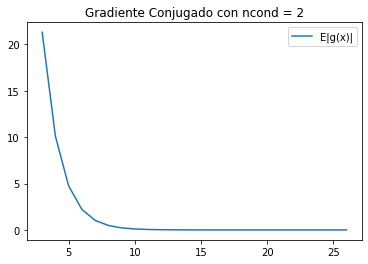
\includegraphics[width=0.7\linewidth]{graficas/gc_2}
\end{center}

\begin{center}
	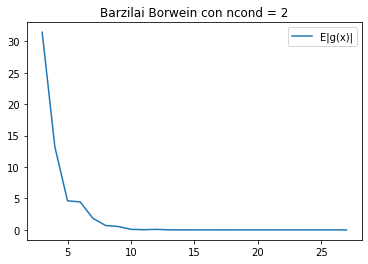
\includegraphics[width=0.7\linewidth]{graficas/bb_2}
	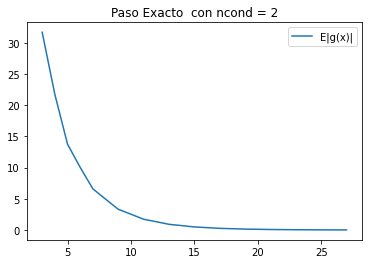
\includegraphics[width=0.7\linewidth]{graficas/sd_2}
\end{center}


\subsubsection{$ ncond = 4 $}

\begin{center}
	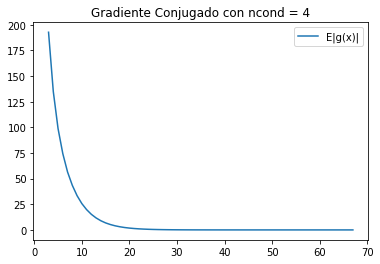
\includegraphics[width=0.7\linewidth]{graficas/gc_4}
	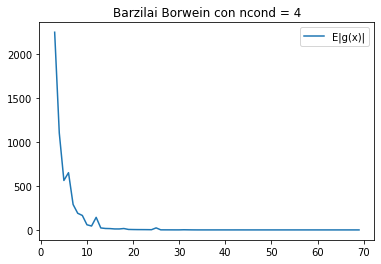
\includegraphics[width=0.7\linewidth]{graficas/bb_4}
	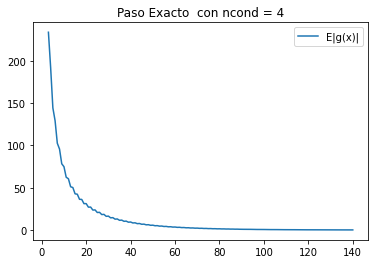
\includegraphics[width=0.7\linewidth]{graficas/sd_4}
\end{center}
\subsubsection{$ ncond = 6 $}

\begin{center}
	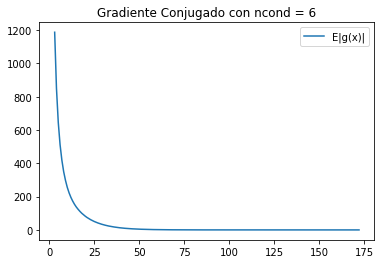
\includegraphics[width=0.7\linewidth]{graficas/gc_6}
	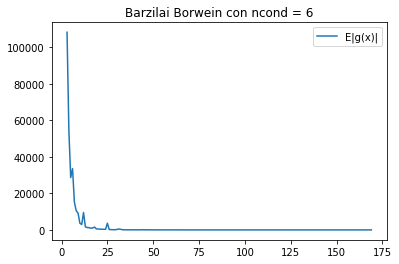
\includegraphics[width=0.7\linewidth]{graficas/bb_6}
	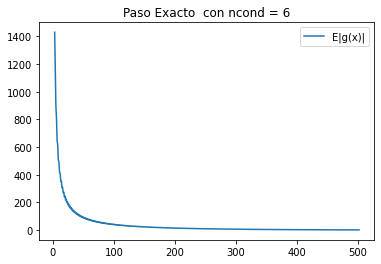
\includegraphics[width=0.7\linewidth]{graficas/sd_6}
\end{center}
\section{Conclusiones}
	\subsection{Gradiente Conjugado}
	Este método utiliza la idea de diagonalizar la matriz $ Q $ para resolver el problema como en el caso base de $ \mathbb{R}^2 $ a través de usar la $ Q $- conjugación. Una característica particular de este método es que genera vectores $ p_0, p_1, \dots, p_k $ tal que cada uno de ellos cumple ser conjugado con la matriz $ Q $ y además este conjunto de vectores son mutuamente ortogonales y linealmente independientes. Para la forma cuadrática dada el algoritmo mostró rendimiento superior en términos de tiempo e iteraciones respecto al algoritmo de paso exacto. Notemos además, que conforme el número de condición se aumenta, el número de iteraciones crece para todos los algoritmos. Esto se ve reflejado en la matriz $ D $ y por lo tanto en $ Q = P^T D P $ , es decir, si $ ncond $ crece, las entradas de $ D $ crecen en valor absoluto y también crecen las entradas de $ Q $. 
	\subsection{Barzilai-Borwein}
	Para la forma cuadrática dada el algoritmo fue el mejor en términos de tiempo e iteraciones. Este método utiliza la idea de aproximar la matriz Hessiana utilizando solamente el gradiente. Lo anterior explica por qué el rendimiento fue superior, dado que no solamente trata de utilizar información del gradiente si no que incorpora información aportada por el Hessiano.
	\subsection{Paso Exacto}
	Este algoritmo es de los primeros visto en clases. Para el caso de una forma cuadrática dada, se conoce la expresión para el paso $ \alpha_k $. Notemos que de los tres métodos utilizados este fue el más lento respecto a tiempo e iteraciones. 
\end{document}